%% ----------------------------------------------------------------
%% Introduction.tex
%% ---------------------------------------------------------------- 
\chapter{Introduction} \label{Chapter:Introduction}

This dissertation was a part of my master’s project at the Univerisity of Southampton, under the guidance of Dr. Sasan Barak. The project focuses on financial data science within cryptocurrency markets. 

Financial markets, like cryptocurrencies, are widely considered to be non-stationary~\cite{Schmitt_2013,Lo} as their statistical properties—including volatility, correlations, and return distributions change frequently over time.
The non-stationarity brings a major challenge for trading and risk management, as optimised strategies under one regime often fail when market condition changes~\cite{10.1093/rfs/15.4.1137}. 

Traditional trading strategies generally assume a stable market environment, therefore the strategy performance probably varies across different market states. For example, a momentum-based method may perform well in a trending market but much worse in volatile periods~\cite{MOSKOWITZ2012228}; Similarly, risk measures calculated under a volatility regime may underestimate the risk during a crisis regime~\cite{HAMILTON1994307}.

To address the challenges from market non-stationarity, a range of methods are developed, such as Markov switching models~\cite{hamilton1989new}, and clustering approaches~\cite{10.1093/rfs/15.4.1137}. More recently, mathematical tools from rough path theory have given rise to signature methods~\cite{ chevyrev2025primersignaturemethodmachine,issa2023nonparametriconlinemarketregime}, which are capable of extracting rich path-wise features from time series data. Combined with clustering, these features can be used to identify distinct market regimes, such as bull, bear, and neutral phases.

In this study, we applied signature methods~\cite{Lyons1998, chevyrev2025primersignaturemethodmachine,issa2023nonparametriconlinemarketregime} to extract path-wise features from BTC prices and perform walk-forward clustering to obtain bull/neutral/bear regimes. We then applied a cross-sectional lead–lag hedge~\cite{lyons2002system, gatheral2018volatility} as the baseline and overlay the regime signal to adjust position signs and exposure.


The main contributions of this dissertation can be summarised in three parts. First, it shows how signature methods can be used for regime detection in cryptocurrency markets, which is still a relatively new application. Second, it develops a framework that combines regime signals with trading strategies, taking the lead–lag strategy as the baseline. Third, it provides a comparative evaluation between the baseline strategy and its regime-aware extension, showing the benefits in risk–return trade-offs as well as the limits of the application.

The dissertation is organised as follows. Chapter 2 reviews the relevant literature on financial market non-stationarity, regime detection methods, and cryptocurrency trading strategies. Chapter 3 introduces the methodology, including signature methods, clustering techniques, and the construction of baseline and regime-aware strategies. Chapter 4 presents the empirical results and performance evaluation. Chapter 5 discusses the limitations and potential extensions, including multi-asset regimes and transaction cost considerations. Finally, Chapter 6 concludes with a summary of contributions and directions for future research.

%The lead–lag effect \cite{Podobnik_2010} is about timing — when changes in one time series tend to show up before similar changes in another. An illustration of this in financial markets is that some assets shows predictable movements because their price changes tend to follow those of other assets after a certain time lag \cite{huth2012highfrequencyleadlagrelationships,repec:taf:quantf:v:18:y:2018:i:5:p:725-735}. The study of lead-lag relationships between asset returns can help active investors build trading algorithms that exploit the time lag in the movement of one asset relative to another and generate strong returns \cite{Li2022}.

\iffalse
Many methods are developed to detect the lead-lag relationship

You probably found all the files from \cite{Gunn:2001:pdflatex}.
\tref{Table:tabex} illustrates the results of my work.
\begin{table}[!htb]
  \centering
  \begin{tabular}{cc}
  \toprule
  \textbf{Training Error} & \textbf{Testing Error}\\
  \midrule
  0 & $\infty$\\
  \bottomrule
  \end{tabular}
  \caption{The Results}
  \label{Table:tabex}
\end{table}

\fref{Figure:figex} shows why this is the case.
\begin{figure}[!htb]
  \centering
  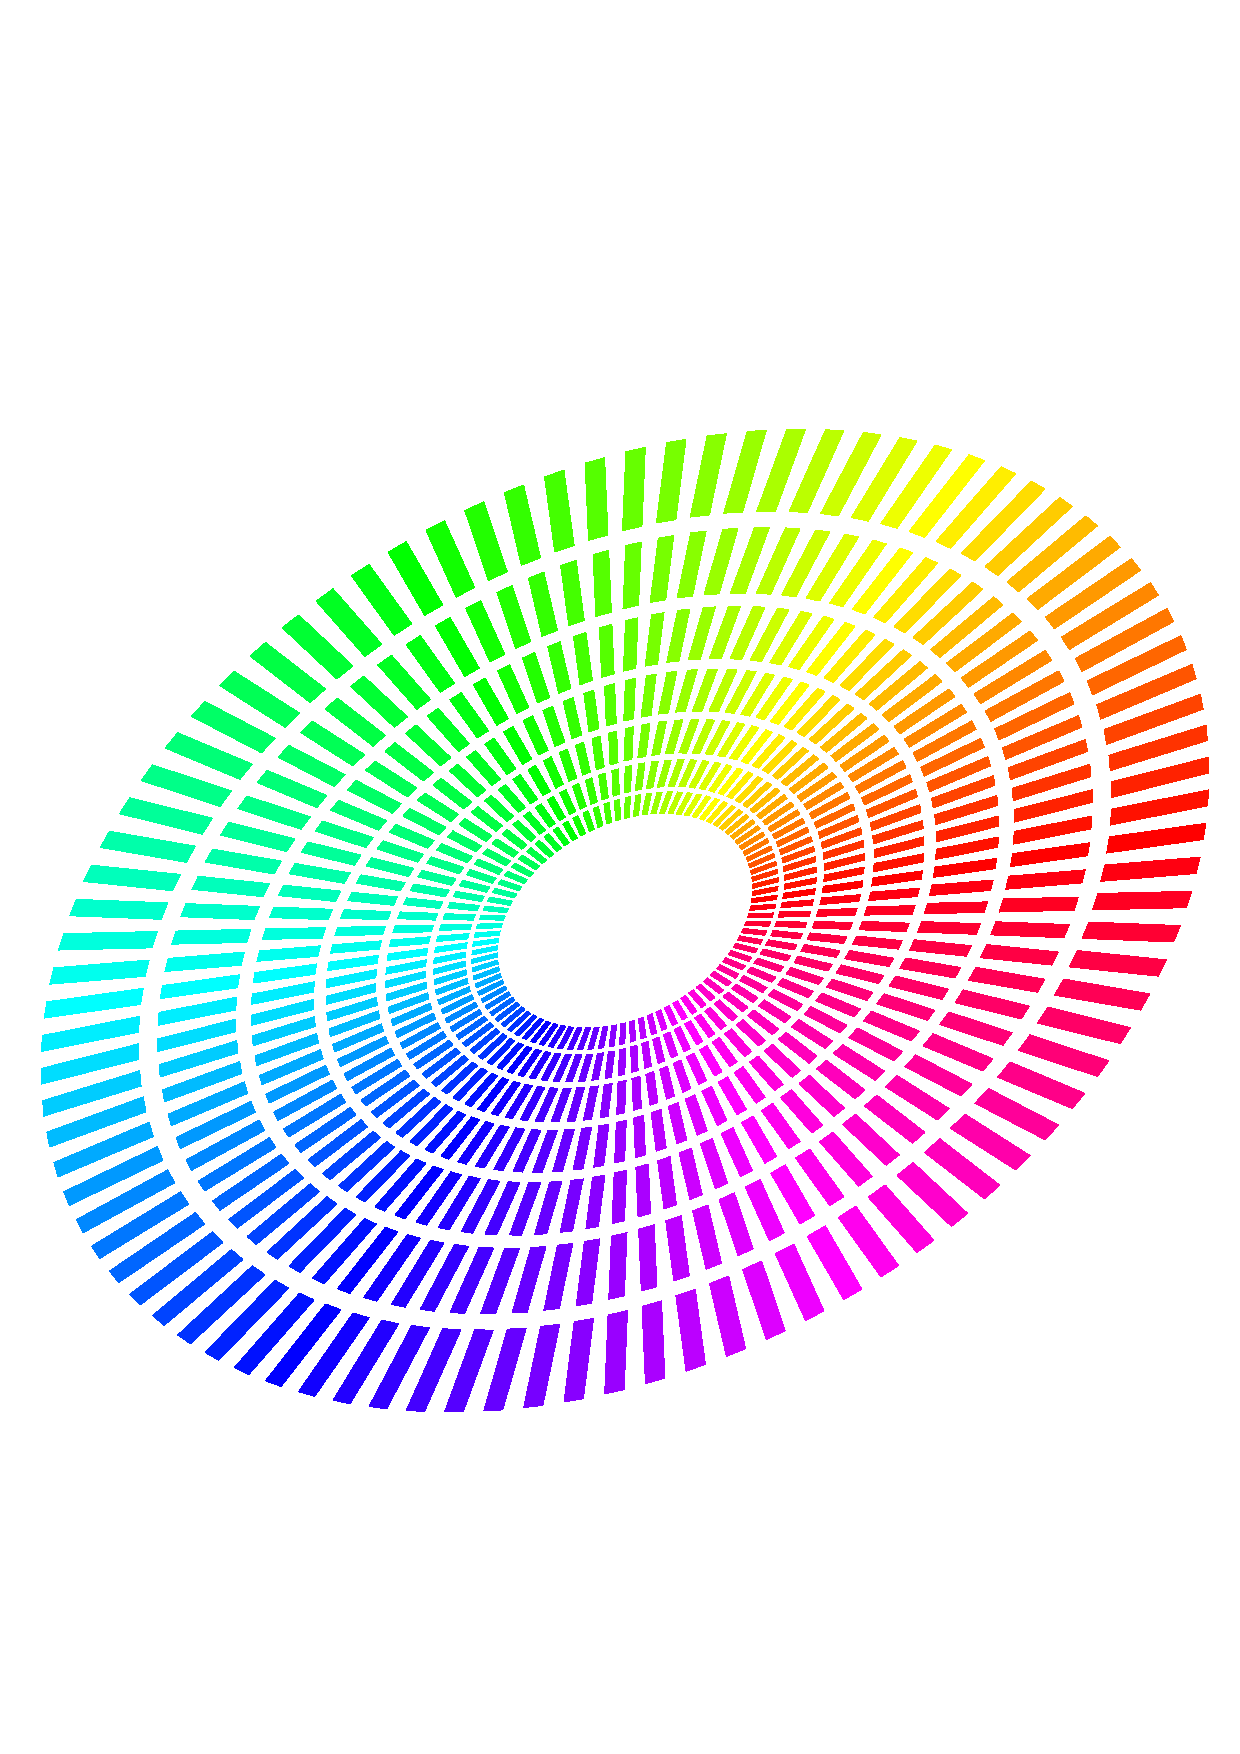
\includegraphics[width=8cm]{figure}
  \caption{A colourful picture.}
  \label{Figure:figex}
\end{figure}

This page shows you a subfigure example in \fref{Figure:figsubex}.
\begin{figure}[!htb]
  \centering
  \subfigure[The left caption]{
    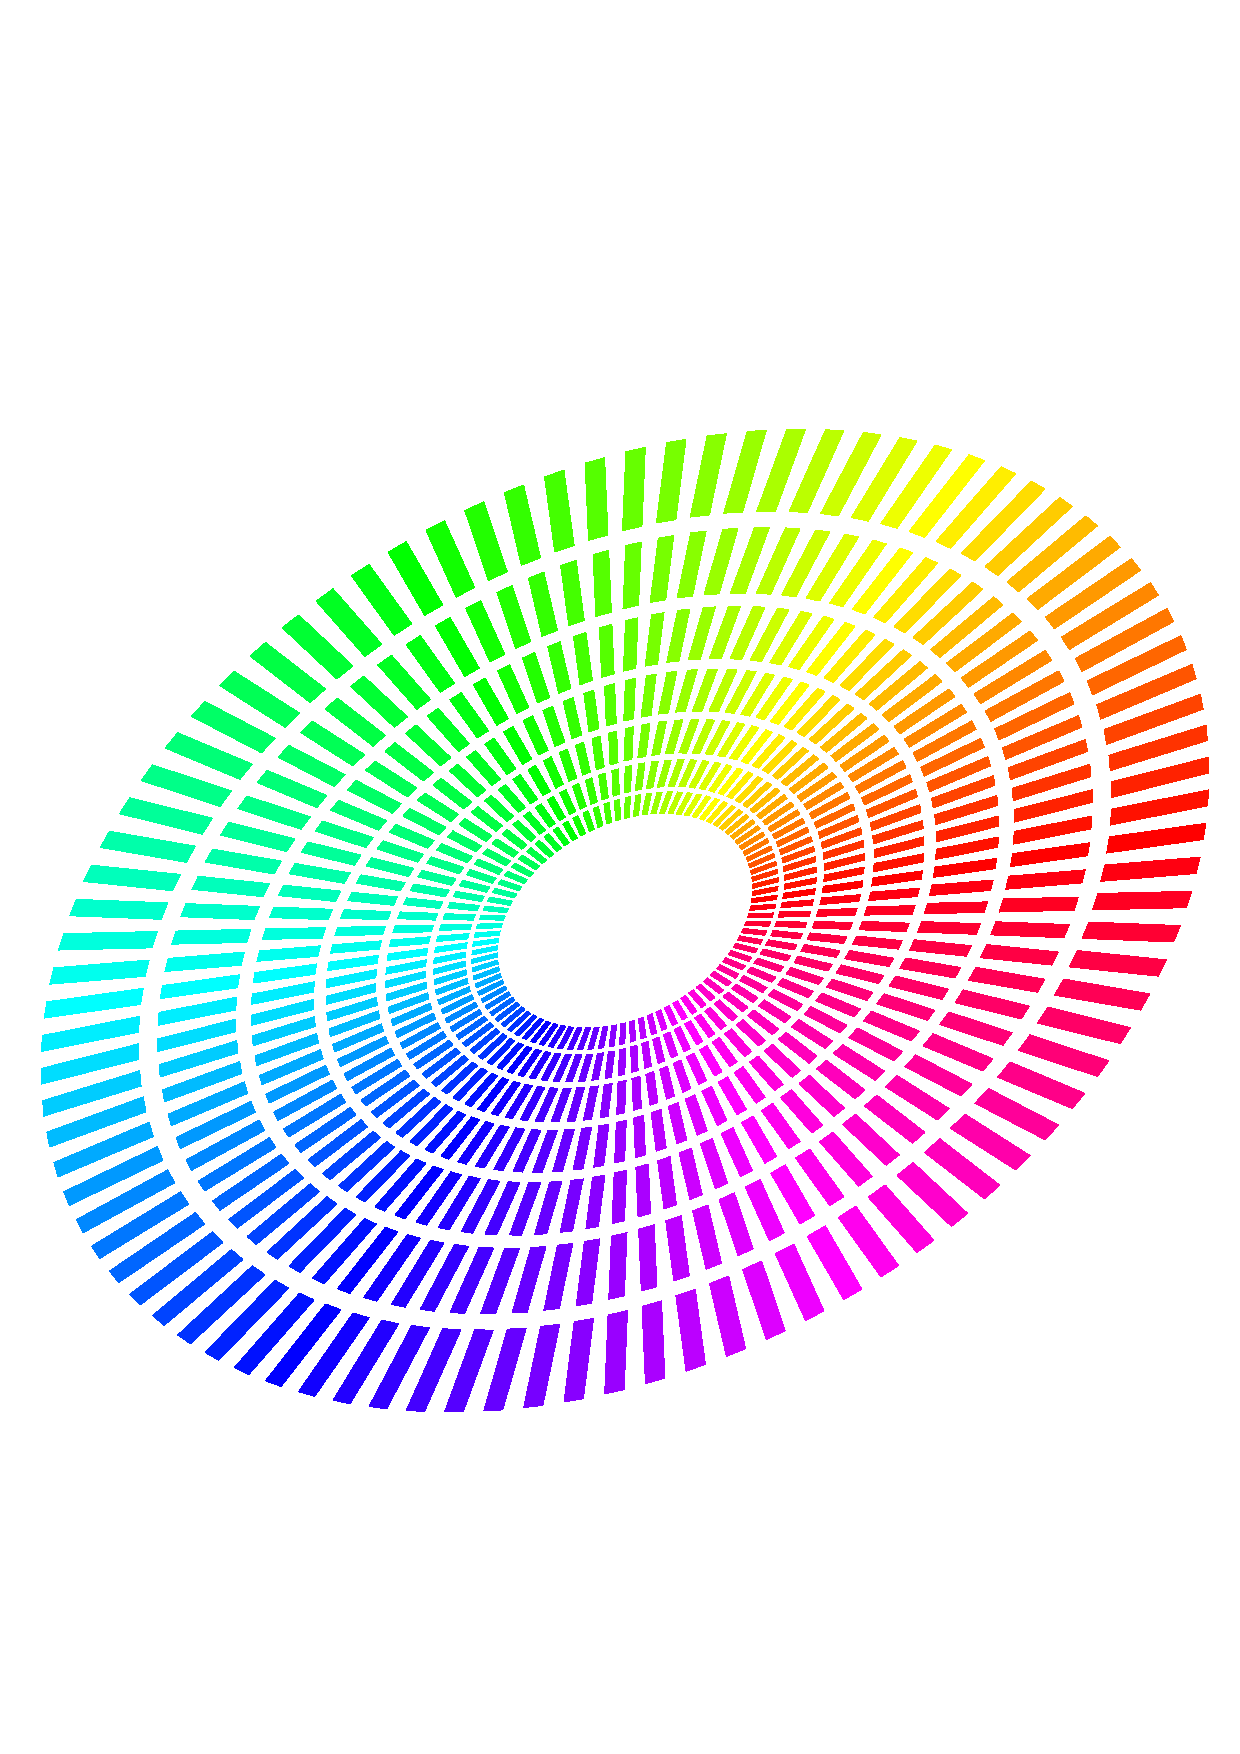
\includegraphics[width=4.2cm]{figure}
    \label{Figure:figsubex:left}
  }
  \subfigure[The right caption]{
    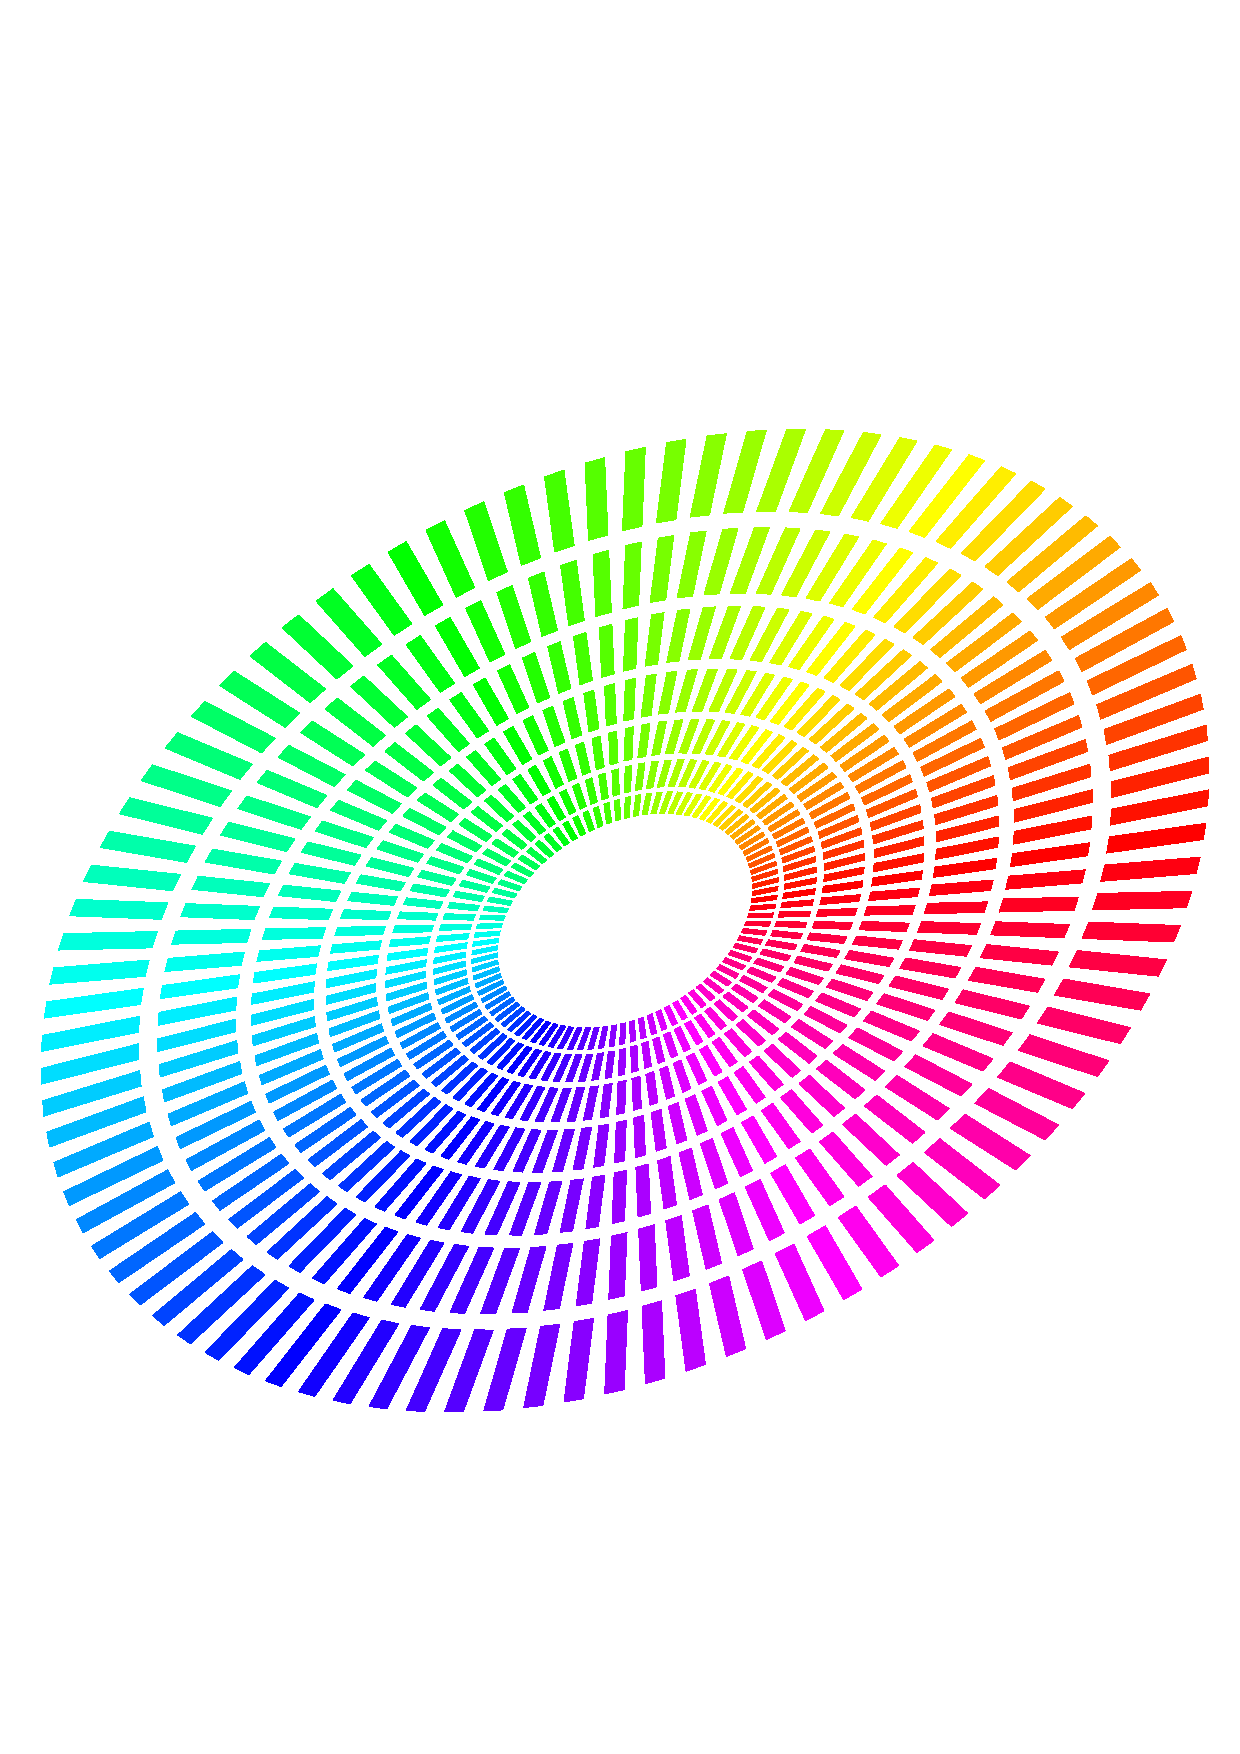
\includegraphics[width=4.2cm]{figure}
    \label{Figure:figsubex:right}
  }
  \caption{A doubly colourful picture.}
  \label{Figure:figsubex}
\end{figure}
\fi